\documentclass[aspectratio=169]{beamer}
\usepackage[utf8]{inputenc}

% design
\usetheme{CambridgeUS}
\usecolortheme{beaver}
\setbeamertemplate{itemize items}[square]
\usenavigationsymbolstemplate{\beamertemplatenavigationsymbolsempty}
\definecolor{darkred}{rgb}{0.8,0,0}
\setbeamertemplate{enumerate item}{\color{darkred}\insertenumlabel.}
\setbeamertemplate{itemize item}{\color{darkred}$\blacktriangleright$}
\setlength{\tabcolsep}{12pt}
\setbeamercolor{block title}{fg=darkred}

% bibliography
%\usepackage[backend=biber, style=authortitle]{biblatex}
\usepackage{natbib}
\usepackage{har2nat}
\bibliographystyle{unsrt}
%\addbibresource{../../smc.bib}
\usepackage{bibentry}
\nobibliography*

% tikz
\usepackage{tikz}
\usetikzlibrary{positioning}

% maths
\usepackage{amsmath}
\usepackage{amssymb}
\usepackage{amsfonts}
\usepackage{amsthm}
\theoremstyle{definition}
\newtheorem{defn}{Definition}

% useful math symbols
\newcommand{\PR}{\mathbb{P}}
\newcommand{\E}{\mathbb{E}}
\newcommand{\V}{\operatorname{Var}}
\newcommand{\eqdist}{\overset{d}{=}}
\newcommand{\I}[1]{\mathbb{I}\{#1\}}
\newcommand{\Ntoinfty}{\overset{N\to\infty}{\longrightarrow}}
\newcommand{\limNtoinfty}{\underset{N\to\infty}{\lim}}
\newcommand\indep{\protect\mathpalette{\protect\independenT}{\perp}}
\def\independenT#1#2{\mathrel{\rlap{$#1#2$}\mkern2mu{#1#2}}}

% distributions
\newcommand{\N}{\mathcal{N}}
\newcommand{\Cat}{\operatorname{Categorical}}
\newcommand{\Unif}{\operatorname{Uniform}}
\newcommand{\Mn}{\operatorname{Multinomial}}
\newcommand{\Bin}{\operatorname{Binomial}}

% project-specific commands
\newcommand{\F}{\mathcal{F}_{t-1}}
\newcommand{\vt}[2][t]{v_{#1}^{(#2)}}
%\newcommand{\vt}[1]{v_{#1}}
\newcommand{\wt}[2][t]{w_{#1}^{(#2)}}
%\newcommand{\wt}[1]{w_{#1}}
%\newcommand{\wbar}[2][t]{\bar{w}_{#1}^{(#2)}}
%\newcommand{\vttilde}[2][t]{\tilde{v}_{#1}^{(#2)}}
\newcommand{\Et}{\mathbb{E}_{t}}

\title[Genealogies of SMC Algorithms]{Asymptotic genealogies of sequential Monte Carlo algorithms}
\author[Suzie Brown]{\textbf{Suzie Brown} \\ University of Warwick \\ with Paul Jenkins, Adam Johansen \& Jere Koskela}
\date{18 November 2020} 

\begin{document}
\begin{frame}
\maketitle
\end{frame}

\begin{frame}{Outline}
\begin{enumerate}
\item ...
\end{enumerate}
\end{frame}

%% add a frame with SMC algm skeleton, to fix notation g,q etc.?

\begin{frame}{Sequential Monte Carlo}
\centering
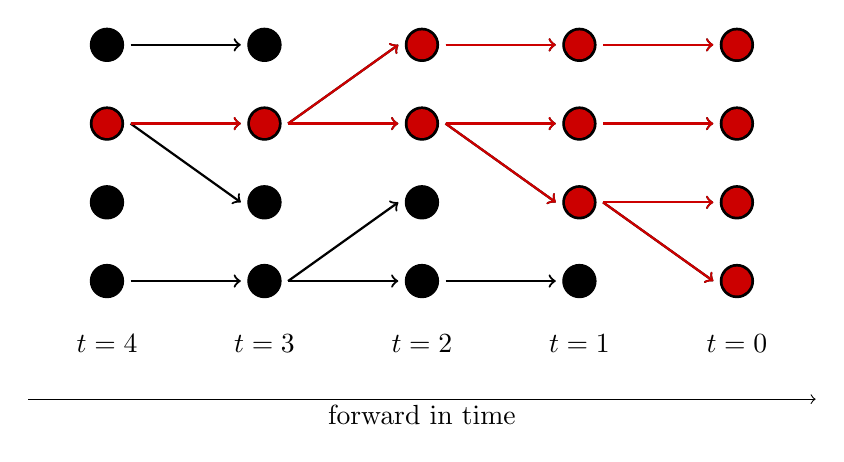
\begin{tikzpicture}
\filldraw (0,0) circle (6pt);
\filldraw (0,-1) circle (6pt);
\filldraw (0,-2) circle (6pt);
\filldraw (0,-3) circle (6pt);

\draw[->] (-1,-4.5)--(9,-4.5);
\node at (4,-4.7) {forward in time};

\filldraw (2,0) circle (6pt);
\filldraw (2,-1) circle (6pt);
\filldraw (2,-2) circle (6pt);
\filldraw (2,-3) circle (6pt);

\filldraw (4,0) circle (6pt);
\filldraw (4,-1) circle (6pt);
\filldraw (4,-2) circle (6pt);
\filldraw (4,-3) circle (6pt);

\filldraw (6,0) circle (6pt);
\filldraw (6,-1) circle (6pt);
\filldraw (6,-2) circle (6pt);
\filldraw (6,-3) circle (6pt);

\filldraw (8,0) circle (6pt);
\filldraw (8,-1) circle (6pt);
\filldraw (8,-2) circle (6pt);
\filldraw (8,-3) circle (6pt);

\draw[->, thick] (0.3,0)--(1.7,0);
\draw[->, thick] (0.3,-1)--(1.7,-1);
\draw[->, thick] (0.3,-3)--(1.7,-3);
\draw[->, thick] (0.3,-1)--(1.7,-2);

\draw[->, thick] (2.3,-1)--(3.7,0);
\draw[->, thick] (2.3,-1)--(3.7,-1);
\draw[->, thick] (2.3,-3)--(3.7,-2);
\draw[->, thick] (2.3,-3)--(3.7,-3);

\draw[->, thick] (4.3,0)--(5.7,0);
\draw[->, thick] (4.3,-1)--(5.7,-1);
\draw[->, thick] (4.3,-1)--(5.7,-2);
\draw[->, thick] (4.3,-3)--(5.7,-3);

\draw[->, thick] (6.3,0)--(7.7,0);
\draw[->, thick] (6.3,-1)--(7.7,-1);
\draw[->, thick] (6.3,-2)--(7.7,-2);
\draw[->, thick] (6.3,-2)--(7.7,-3);

\pause
\node at (8,-3.8) {$t=0$};
\pause
\node at (6,-3.8) {$t=1$};
\node at (4,-3.8) {$t=2$};
\node at (2,-3.8) {$t=3$};
\node at (0,-3.8) {$t=4$};

\pause
% highlight first lineage
\filldraw[darkred] (8,0) circle (5pt);
\pause
\filldraw[darkred] (6,0) circle (5pt);
\filldraw[darkred] (4,0) circle (5pt);
\filldraw[darkred] (2,-1) circle (5pt);
\filldraw[darkred] (0,-1) circle (5pt);

\draw[->, thick, darkred] (0.3,-1)--(1.7,-1);
\draw[->, thick, darkred] (2.3,-1)--(3.7,0);
\draw[->, thick, darkred] (4.3,0)--(5.7,0);
\draw[->, thick, darkred] (6.3,0)--(7.7,0);

\pause
% highlight other lineages
\filldraw[darkred] (4,-1) circle (5pt);
\filldraw[darkred] (6,-1) circle (5pt);
\filldraw[darkred] (8,-1) circle (5pt);
\filldraw[darkred] (6,-2) circle (5pt);
\filldraw[darkred] (8,-2) circle (5pt);
\filldraw[darkred] (8,-3) circle (5pt);

\draw[->, thick, darkred] (2.3,-1)--(3.7,-1);
\draw[->, thick, darkred] (4.3,-1)--(5.7,-1);
\draw[->, thick, darkred] (4.3,-1)--(5.7,-2);
\draw[->, thick, darkred] (6.3,-1)--(7.7,-1);
\draw[->, thick, darkred] (6.3,-2)--(7.7,-2);
\draw[->, thick, darkred] (6.3,-2)--(7.7,-3);
\end{tikzpicture}
\end{frame}

\begin{frame}{Induced genealogy}
\centering
\begin{tikzpicture}
\draw[dotted] (0,-4.5)--(0,0.5);
\draw[dotted] (2,-4.5)--(2,0.5);
\draw[dotted] (4,-4.5)--(4,0.5);
\draw[dotted] (6,-4.5)--(6,0.5);
\draw[dotted] (8,-4.5)--(8,0.5);

\draw[thick, darkred] (0,-1)--(2,-1);
\draw[thick, darkred] (2,0)--(2,-2);
\draw[thick, darkred] (2,0)--(8,0);
\draw[thick, darkred] (2,-2)--(4,-2);
\draw[thick, darkred] (4,-3)--(4,-1);
\draw[thick, darkred] (4,-1)--(8,-1);
\draw[thick, darkred] (4,-3)--(6,-3);
\draw[thick, darkred] (6,-2)--(6,-4);
\draw[thick, darkred] (6,-2)--(8,-2);
\draw[thick, darkred] (6,-4)--(8,-4);

\node at (8,-4.8) {$t=0$};
\node at (6,-4.8) {$t=1$};
\node at (4,-4.8) {$t=2$};
\node at (2,-4.8) {$t=3$};
\node at (0,-4.8) {$t=4$};
\end{tikzpicture}
\end{frame}

\begin{frame}{Mathematical formulation}
\begin{itemize}
\item Population of $N$ particles
\item Sample $n\leq N$ terminal particles
\pause
\item Describe genealogy by a partition-valued stochastic process $(G_t^{(n,N)})_{t\in\mathbb{N}_0}$
\item Elements $i, j$ are in the same block of the partition $G_t^{(n,N)}$ iff particles $i$ and $j$ share a common ancestor at time $t$
\pause
\item At time 0, the partition of $\{1,\dots,n\}$ consisting of singletons: $G_0^{(n,N)} = \{ \{1\}, \dots, \{n\} \}$
\item The only possible non-identity transitions are those that merge blocks
\end{itemize}

\end{frame}

\begin{frame}{Example}
\centering
\begin{tikzpicture}
\draw[dotted] (0,-4.5)--(0,0.5);
\draw[dotted] (2,-4.5)--(2,0.5);
\draw[dotted] (4,-4.5)--(4,0.5);
\draw[dotted] (6,-4.5)--(6,0.5);
\draw[dotted] (8,-4.5)--(8,0.5);

\draw[thick, darkred] (0,-1)--(2,-1);
\draw[thick, darkred] (2,0)--(2,-2);
\draw[thick, darkred] (2,0)--(8,0);
\draw[thick, darkred] (2,-2)--(4,-2);
\draw[thick, darkred] (4,-3)--(4,-1);
\draw[thick, darkred] (4,-1)--(8,-1);
\draw[thick, darkred] (4,-3)--(6,-3);
\draw[thick, darkred] (6,-2)--(6,-4);
\draw[thick, darkred] (6,-2)--(8,-2);
\draw[thick, darkred] (6,-4)--(8,-4);

\node at (8.3,0) {1};
\node at (8.3,-1) {2};
\node at (8.3,-2) {3};
\node at (8.3,-4) {4};

\node at (8,-4.8) {$t=0$};
\node at (8,-5.5) {$\{1\}, \{2\},\{3\}, \{4\}$};
\end{tikzpicture}
\end{frame}

\begin{frame}{Example}
\centering
\begin{tikzpicture}
\draw[dotted] (0,-4.5)--(0,0.5);
\draw[dotted] (2,-4.5)--(2,0.5);
\draw[dotted] (4,-4.5)--(4,0.5);
\draw[dotted] (6,-4.5)--(6,0.5);
\draw[dotted] (8,-4.5)--(8,0.5);

\draw[thick, darkred] (0,-1)--(2,-1);
\draw[thick, darkred] (2,0)--(2,-2);
\draw[thick, darkred] (2,0)--(8,0);
\draw[thick, darkred] (2,-2)--(4,-2);
\draw[thick, darkred] (4,-3)--(4,-1);
\draw[thick, darkred] (4,-1)--(8,-1);
\draw[thick, darkred] (4,-3)--(6,-3);
\draw[thick, darkred] (6,-2)--(6,-4);
\draw[thick, darkred] (6,-2)--(8,-2);
\draw[thick, darkred] (6,-4)--(8,-4);

\node at (8.3,0) {1};
\node at (8.3,-1) {2};
\node at (8.3,-2) {3};
\node at (8.3,-4) {4};

\node at (6,-4.8) {$t=1$};
\node at (6,-5.5) {$\{1\}, \{2\},\{3,4\}$};
\end{tikzpicture}
\end{frame}

\begin{frame}{Example}
\centering
\begin{tikzpicture}
\draw[dotted] (0,-4.5)--(0,0.5);
\draw[dotted] (2,-4.5)--(2,0.5);
\draw[dotted] (4,-4.5)--(4,0.5);
\draw[dotted] (6,-4.5)--(6,0.5);
\draw[dotted] (8,-4.5)--(8,0.5);

\draw[thick, darkred] (0,-1)--(2,-1);
\draw[thick, darkred] (2,0)--(2,-2);
\draw[thick, darkred] (2,0)--(8,0);
\draw[thick, darkred] (2,-2)--(4,-2);
\draw[thick, darkred] (4,-3)--(4,-1);
\draw[thick, darkred] (4,-1)--(8,-1);
\draw[thick, darkred] (4,-3)--(6,-3);
\draw[thick, darkred] (6,-2)--(6,-4);
\draw[thick, darkred] (6,-2)--(8,-2);
\draw[thick, darkred] (6,-4)--(8,-4);

\node at (8.3,0) {1};
\node at (8.3,-1) {2};
\node at (8.3,-2) {3};
\node at (8.3,-4) {4};

\node at (4,-4.8) {$t=2$};
\node at (4,-5.5) {$\{1\}, \{2,3,4\}$};
\end{tikzpicture}
\end{frame}

\begin{frame}{Example}
\centering
\begin{tikzpicture}
\draw[dotted] (0,-4.5)--(0,0.5);
\draw[dotted] (2,-4.5)--(2,0.5);
\draw[dotted] (4,-4.5)--(4,0.5);
\draw[dotted] (6,-4.5)--(6,0.5);
\draw[dotted] (8,-4.5)--(8,0.5);

\draw[thick, darkred] (0,-1)--(2,-1);
\draw[thick, darkred] (2,0)--(2,-2);
\draw[thick, darkred] (2,0)--(8,0);
\draw[thick, darkred] (2,-2)--(4,-2);
\draw[thick, darkred] (4,-3)--(4,-1);
\draw[thick, darkred] (4,-1)--(8,-1);
\draw[thick, darkred] (4,-3)--(6,-3);
\draw[thick, darkred] (6,-2)--(6,-4);
\draw[thick, darkred] (6,-2)--(8,-2);
\draw[thick, darkred] (6,-4)--(8,-4);

\node at (8.3,0) {1};
\node at (8.3,-1) {2};
\node at (8.3,-2) {3};
\node at (8.3,-4) {4};

\node at (2,-4.8) {$t=3$};
\node at (2,-5.5) {$\{1,2,3,4\}$};
\end{tikzpicture}
\end{frame}

\begin{frame}{Kingman's $n$-coalescent}
\begin{itemize}
\pause
\item $n$ terminal particles
\item Continuous time
\item Each pair of lineages coalesces at rate 1
\item No other ($>$ pair) mergers allowed
\end{itemize}
\end{frame}

\begin{frame}{Notation}
\begin{itemize}
\item $\wt{i}$ = weight of particle $i$ in generation $t$
\item family size $\vt{i}$ = number of offspring of particle $i$ in generation $t$
\pause
\item pair merger probability $c_N(t) = \frac{1}{N(N-1)}\sum_{i=1}^N \vt{i}(\vt{i}-1)$
\pause
\item time scale $\tau_N(t)$ = inverse of $c_N(t)$
\end{itemize}
\end{frame}

\begin{frame}{A convergence theorem\footnote{Koskela, Jenkins, Johansen, Span\`o. \textit{Ann Stat,} to appear.}}
\vspace{-10pt}
Suppose:
\begin{align*}
\E [c_N(t)] &\rightarrow 0  \\
\E \left[ \sum_{ r = \tau_N( s ) + 1 }^{ \tau_N( t ) } D_N( r ) \right] &\rightarrow 0 \\
\E \left[ \sum_{ r = \tau_N( s ) + 1 }^{ \tau_N( t ) } c_N( r )^2 \right] &\rightarrow 0 \\
\E [\tau_N(t) - \tau_N(s)] &\leq C_{t,s} N 
\end{align*}
Then the rescaled genealogical process $(G_{\tau_N(t)}^{(n,N)})_{t\geq0} $ converges to Kingman's coalescent in the sense of finite-dimensional distributions as $N\to\infty$.
\end{frame}

\begin{frame}{A simplified statement}
\vspace{-10pt}
\pause
Suppose there exists a deterministic sequence $(b_N)_{N\in\mathbb{N}}$ uniform in $t\geq 1$ such that $b_N \to 0$.
\begin{equation*}
\frac{1}{N(N-1)(N-2)} \sum_{i = 1}^N \Et[ \vt{i}(\vt{i}-1)(\vt{i}-2) ]  \leq b_N \frac{1}{N(N-1)} \sum_{i = 1}^N \Et[ \vt{i}(\vt{i}-1)  ]
\end{equation*}

Then the rescaled genealogical process $(G_{\tau_N(t)}^{(n,N)})_{t\geq0} $ converges to Kingman's coalescent in the sense of finite-dimensional distributions as $N\to\infty$.
\end{frame}

\begin{frame}{Remarks}
\begin{itemize}
\item We replace four conditions with one
\pause
\item We remove condition 4, which we know is not a necessary condition
\pause
\item We remove conditions 2 and 3, which contain awkward mixed moments
\pause
\item We can verify the new condition in more complicated cases...
\end{itemize}
\end{frame}

\begin{frame}{Resampling schemes}
Problem : (stochastically) map weights $(\wt{1}, \dots, \wt{N})$ to family sizes $(\vt{1},\dots, \vt{N})$.\\

\pause
Desirable properties:
\begin{itemize}
\item Number of particles constant $\sum_{i=1}^N \vt{i} =N$
\item Equal weights after resampling $w_{t+}^{(i)} = 1/N$
\item Unbiased $\E[\vt{i} | \wt{i}] = N\wt{i}$
\end{itemize}
\end{frame}

\begin{frame}{Corollary: multinomial resampling}
Consider an SMC algorithm with potential $g$ and transition density $q$, satisfying
\begin{align*}
\frac{1}{a} \leq &g_t(x, x^\prime) \leq a \\
\varepsilon h(x^\prime) \leq &q_t(x, x^\prime) \leq \frac{1}{\varepsilon} h(x^\prime) 
\end{align*}
for constants $0<\varepsilon\leq 1\leq a<\infty$, and probablity distribution $h(\cdot)$.\\[10pt]

Under multinomial resampling, the rescaled genealogies converge to Kingman's coalescent.
\end{frame}

\begin{frame}{Stochastic roundings}
\pause
Let $X\geq 0$.\\
$Y: \mathbb{R}_+ \to \mathbb{N}$ is a \emph{stochastic rounding} of $X$ if $Y$ takes the values
\begin{equation*}
Y \mid X =
\begin{cases}
 \lfloor X \rfloor & \text{with probability } 1- X+ \lfloor X \rfloor \\
  \lfloor X \rfloor +1 & \text{with probability } X- \lfloor X \rfloor 
\end{cases}
\end{equation*}
\pause
Can generalise to multivariate case, with marginals $Y_i \mid X_i$ as above.
\end{frame}

\begin{frame}{Stochastic roundings}
\begin{itemize}
\item $X_i = N\wt{i}$
\item $\vt{i} = Y_i$
\item Constraint $Y_1+\dots +Y_N = N$
\pause
\item Examples: systematic resampling, residual-stratified resampling, SSP resampling\footnote{Gerber, Whiteley, Chopin. \textit{Ann Stat,} 2019.},...
\end{itemize}
\end{frame}

\begin{frame}{Corollary: stochastic rounding -based resampling}
Consider an SMC algorithm with potential $g$ and transition density $q$, satisfying
\begin{align*}
\frac{1}{a} \leq &g_t(x, x^\prime) \leq a \\
\varepsilon h(x^\prime) \leq &q_t(x, x^\prime) \leq \frac{1}{\varepsilon} h(x^\prime) 
\end{align*}
for constants $0<\varepsilon\leq 1\leq a<\infty$, and probablity distribution $h(\cdot)$.\\[10pt]

Under stochastic rounding -based resampling, the rescaled genealogies converge to Kingman's coalescent.
\end{frame}

\begin{frame}{Conditional SMC}
\begin{itemize}
\item Used for SMC updates in particle MCMC\footnote{Andrieu, Doucet, Holenstein. \textit{JRSSB}, 2010.}
\item Given a fixed ``immortal trajectory'', conditioned to survive all transition and resampling steps
\end{itemize}
\end{frame}

\begin{frame}{Corollary: conditional SMC}
Consider a conditional SMC algorithm with potential $g$ and transition density $q$, satisfying
\begin{align*}
\frac{1}{a} \leq &g_t(x, x^\prime) \leq a \\
\varepsilon h(x^\prime) \leq &q_t(x, x^\prime) \leq \frac{1}{\varepsilon} h(x^\prime) 
\end{align*}
for constants $0<\varepsilon\leq 1\leq a<\infty$, and probablity distribution $h(\cdot)$.\\[10pt]

Under multinomial resampling, the rescaled genealogies converge to Kingman's coalescent.
\end{frame}

\begin{frame}{What about finite $N$?}
\begin{itemize}
\item As $N\to\infty$ but sample size $n$ fixed, probability of sampling immortal line vanishes, so its effect isn't seen in the limit
\pause
\item For finite $N$ we have more interesting behaviour
\item Depends how ``typical'' the immortal trajectory is 
\end{itemize}
\end{frame}

\begin{frame}{Summary}
\begin{itemize}
\item We consider genealogies of SMC algorithms
\item We provide simple conditions for asymptotically Kingman genealogies
\item Satisfied by stochastic rounding -based resampling
\item Satisfied by conditional SMC with multinomial resampling...
\item ... but this hides some interesting pre-limiting behaviour
\end{itemize}
\end{frame}

\end{document}